\documentclass[12pt]{article}
\usepackage{candor, setspace, color}

\usepackage[final, colorlinks=true, linkcolor=BWFBlue,
  citecolor=BWFGreen, urlcolor=BWFRed]{hyperref}
\linespread 2
\numberwithin{equation}{section}

\begin{document}
\tableofcontents

\section{Introduction}

\section{Description of the Model}
\label{allmodel}
\subsection{Free Energy}
\label{freeenergy}

Free energy in a cell arises from the hybridization between two
sequences of RNA and drives ribosomal translation~\cite{starmer}.
\citet{weiss88} suggests the 16S tail of the ribosome hybridizes with its mRNA strand;
from this, we can calculate the free energy values for the interaction between the two strands of RNA.
\citet{freier}, in turn, proposed a thermodynamic model for exactly this,
modeling the interaction in terms of \emph{doublets}: pairs of consecutive nucleotides.
Using this model, Freier calculated the free energy available
for the hybridization of all permutations of RNA doublets.

% Hao: I took out the setting energy values due to irrelevance.
From this, we can simulate hybridization between the associated tRNA, corresponding to the number
of times the force can increment displacement from the current reading frame.
In their deterministic model, the force acts for \emph{exactly} this set number of cycles given a codon.

\subsection{Frameshifts}

% Where the following concept should be first mentioned, I'm not sure -- Vivek

First, we let a displacement of $x = 0$ correspond to the zero reading frame and increments of
\emph{two} to represent a one-nucleotide change. For example, $x =2$ represent the +1 frame.
\citet{lalit:embs} prove that both $x = 0$ and $x = 2$ are fixed (stable) points in displacement in their model,
as would be expected.

\begin{figure}
  \centering
  \caption{Deterministic displacement plot of \prfB}
  \label{prfB:deterministic}
  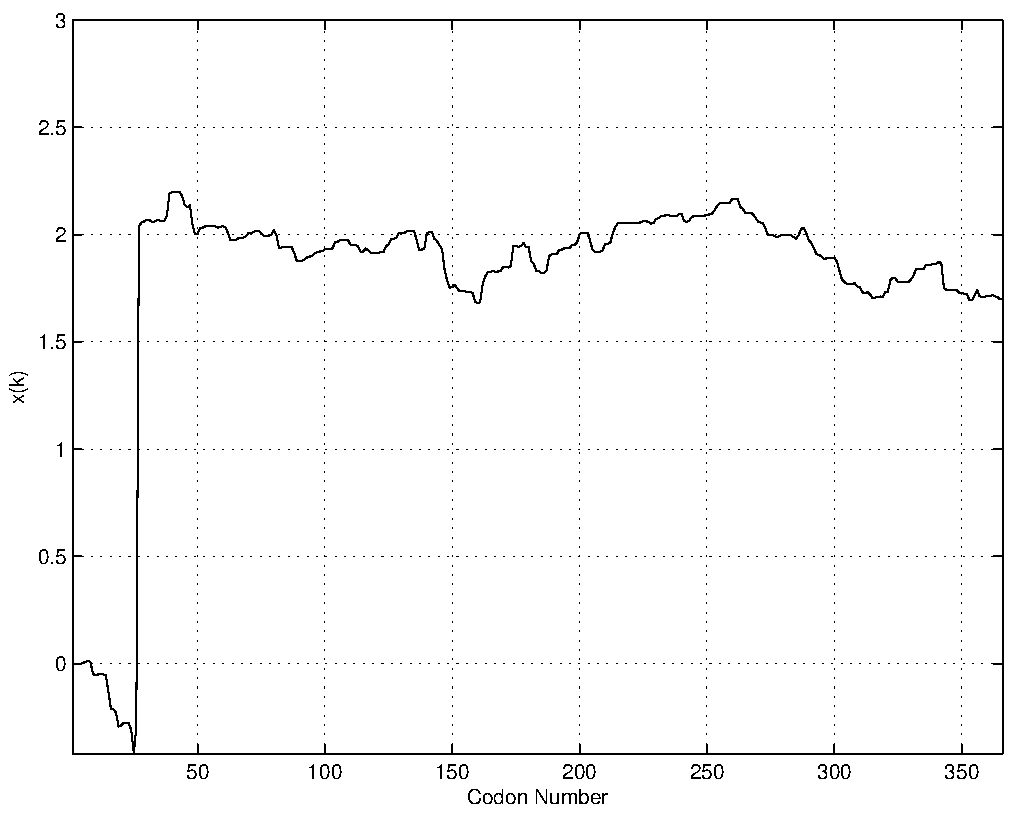
\includegraphics[scale=0.7]{prfB/deterministic.pdf}
\end{figure}

A sudden jump from approximately $x = 0$ to $x = 2$ is then the first indication of a $+1$ frameshift.
In essence, this jump suggests that the ribosome skips one entire base pair in the mRNA sequence.
\autoref{prfB:deterministic} shows the displacement plot per this deterministic model for \prfB, 
a gene known to have a programmed $+1$ frameshift at codon 25.

In conjunction with this characteristic plot, a $+1$ frameshift also shows a clockwise 120\degree\
rotation of phase angle from the species angle, consistent with the creation of displacement data from the phasors.
Intuitively, a frameshift is only sustained if the free energy signal aligns itself with the sudden jump in displacement.
Since the free energy signal has a period of one codon~\cite{lalit:mechanics}, for a $+1$ frameshift the free energy signal
must undergo a phase shift of one-third of an entire period (\autoref{prfb:polar}).

\subsection{A Stochastic Model for Displacement}
\label{stochastic}

% Find an example of a gene with a screwed-up displacement plot under Lalit's old model. --Vivek

As mentioned, the gene \prfB\ exhibits a definite frameshift under the deterministic model: The displacement jumps to $x=2$.
Certain other genes, however, demonstrate ambiguous behavior near $x = \pm 1$.
In a deterministic model, the fixed displacement plots implies
we cannot clearly interpret whether this behavior indicates a tendency for a stable frameshift.
In practice, ribosomal translations are not deterministic. Due to the presence of
noise within the cell environment, we instead chose to model translation stochastically, adding
randomness to the choice of reading frame a ribosome executes at each codon given the free energy signal.
As such, we introduce probability into the model.

We propose that at each cycle in elongation, the ribosome must make a decision: stay in the current reading frame,
move to the $+1$ reading frame,
or move to the $-1$ reading frame.  We can further subdivide this choice into the individual wait-cycles.
At each wait cycle, the ribosome chooses from the above possibilities or proceeds to another wait-cycle without making a decision.

Let $abcd$ be a sequence of four nucleotides, with $abc$ in the
current reading frame and $bcd$ in a +1 reading frame.  Let $x$ be the
displacement of the current wait cycle of the ribosome.  As the
incremental displacement approaches +1, the probability of choosing
codon $bcd$ should increase and the probability of choosing codon
$abc$ should decrease.  We model this behavior using even powers of
cosine and sine functions for $abc$ and $bcd$.  We
define $\omega$ as the \emph{weight} that is directly proportional to
the probability.
\begin{equation}
  \omega_{abc} = \cos^{10}{\frac{x\pi}{4}} \text{ and } \omega_{bcd} = \sin^{10}{\frac{x\pi}{4}}.
\end{equation}
For the purposes of this model, the cosine and sine functions are taken to the tenth power, but
in future studies, this parameter can be modified as long as it stays an even positive integer.
The functions have a period of two base pairs ($x=4$), which is biologically sound:
If the ribosome lies completely in the 0 frame, then the probability of staying in the 0 frame should be 1.  
Consequently, if the ribosome lies fully in the +1 frame ($x=2$), the probability of going to
the 0 frame should be 0.

% DANIEL BEGIN EDIT

Now we define a value $n_{abc}$ based on normalizing $N_{abc}$, the
number of wait cycles, itself inversely proportional to the
tRNA availability of codon $abc$.
We want to wait long enough that the probability of assume the probability of frameshifting after
after $N_{abc}$ wait cycles is $\frac{1}{2}$.  Let $P$ be the
probability of moving on to the next codon and staying in current reading
frame.  Then we should have $1-\left(1-P\right)^{N_{abc}} =
\frac{1}{2}$.  Because $P \propto \omega_{abc}$, we define $n_{abc}$ to be the constant of
proportionality. That is, $n_{abc} = \omega_{abc} / P$.  Coupled
with that $\omega_{abc} \le 1$, we have $n \le \sqrt[N]{2}/(\sqrt[N]{2} - 1).$
where $n = n_{abc}$ and $N = N_{abc}$. Mathematically, the probability of choosing a codon is then
\begin{align}
  \prod_{i=1}^N \left(1-\frac{\omega_i}{n}\right) \text{ where } \omega_i = \cos^{10}{\frac{x_i\pi}{4}}.
\end{align}
Here, $n$ represents the wait time for that codon and $N$ is the ordinal of the wait cycle. (For example,
$N=1$ on the first wait cycle, $N=2$ on the second, and so forth.)
It is important to note that $\omega$ is dependent on displacement, 
which increments after every wait cycle.

% DANIEL END EDIT

\subsection{Measures of Sequence Analysis}

As this model is stochastic, multiple runs of the same sequence must be analyzed.
As such, we propose two metrics for analysis of a number of different runs 
simultaneously. 

\noindent{\textbf{Error-Free Rate.}}  
This metric of analysis is useful when studying a 
sequence with a programmed frameshift.  It measures the percentage of runs 
during which the sequence runs with the ribosome choosing the correct codon
at \emph{every} juncture.  For a +1 frameshift, for example, the ribosome must
choose the +1 frame at the frameshift codon (but must stay in the 0 frame before
and the +1 frame after) in order for the run to be a success.

\noindent{\textbf{Deviation from Baseline.}}
We propose the formula
\begin{equation}
    \label{eqn:lbd}
    d = \sqrt{\frac{\sum_i \left(x_i - \beta_i\right)^2}{N}}
\end{equation}
where $\beta_i$ is the predicted reading frame at codon $i$, $x$ is the displacement at codon $i$,
and $N$ is the total number of codons as a measure of the deviation of the sequence
from the expected reading frame.  Usually $\beta_i = 0$ unless a biologically verified frameshift exists. 
For example, for \prfB\ $\beta_i = 2$ for all $i \geq 25$ because \prfB\ frameshifts at codon 25 (uga)
and the model represents a frameshift with +2 displacement.

This model and all the algorithms that are discussed later in this report
are implemented as a set of MATLAB and Perl codes.  All scripts are available
open-source on the Internet, along with full documentation and many comments.

\section{Calibrating tRNA Availability Values}

\autoref{stochastic} suggests that the stochastic model is dependent
on a number of input parameters, all of which have to be tuned to optimize
the predictive power of the model.  As will be discussed in later sections,
many of these parameters, including the species angle and the initial displacement,
are robust; minor changes in these values will have negligible repercussions
on the output of the model.  A parameter that is much more difficult to estimate
is tRNA availability values (TAV vectors).

\citeauthor{lalit:embs} base the tRNA availability values on codon usage, 
surveying a set of genes from \ecoli.
Although this assumption has biological basis~\cite{ikemura}, 
it is still quite possible that the true values for these numbers may differ 
slightly from those that Ponnala calculated, purely due to sampling error.  
As such, we designed a genetic algorithm to calibrate these values based on the bovine growth hormone (bGH) sequences.
As will be discussed in \autoref{bGH}, biological experiments
have been conducted \cite{schoner:bgh} that propose a set of eight sequences coding for bGH,
two of which have very high yield (pcZ101 and pcZ105) and six of which have low yield.
Since these sequences are known to be translationally regulated, they
provide an excellent method of calibration.

We optimize the separation between pcZ101 and pcZ105 yields and those of other bGH sequences.  
First, we generate a list of randomly modified TAV vectors at which
point we calculate the ratio of the deviation from
displacement (\autoref{deviation}) for pcZ101 and pcZ105 to the other
six bGH proteins. From there, we sort the modified TAV according to
this ratio and discarding the least optimal half of the tRNA
vectors. We then choose two of the remaining vectors, with the chance
of each vector being proportional to its rank.  We then take a
weighted average of the two vectors and spawn a new vector.  After
creating the next generation according to a constant ``gene pool''
size, we delete the previous generation and repeat. After a fixed
number of generations, the algorithm terminates and returns the
optimal TAV vector.

This algorithm did not alter the TAV vectors to a significant degree.
In fact, the average change to each value in the vector was merely
10\%.  Yet, the newly generated vector returns much more optimal
results than the one calculated by \citeauthor{lalit:embs}.  The new values
are used throughout the remainder of the paper to produce the 
values and graphs.

\section{Translational Efficiency}

% Need citations for the following paragraph.

A central problem in modern genetics is that of translational efficiency.
Although most bacteria, like \ecoli, are known to regulate protein production
on the transcriptional level, synthetic genes often encounter translational
problems.  Microbiologists usually resort to trial-and-error to determine genes
that translate at optimal level.  As such, developing a computational method
to roughly predict translational efficiency would have much impact for the 
biological community.

\autoref{allmodel} suggests that divergence from $x=0$ causes
problems in translation; after all, this divergence is an essential characteristic
of a frameshift.  Thus, we stipulate that high translational efficiency should correlate to low deviation yield,
since this requirement implies proximity to the horizontal axis.  This section
evaluates the proposed metric.

\subsection{Ribosomal Proteins}

% CITATION ???

Many microbiologists agree that translation in \ecoli\ is a rather efficient
process.  It logically follows that the model should indicate low deviation
for most \ecoli\ proteins.  Indeed, computational data supports this hypothesis.
\autoref{allhist} is a histogram of the deviation yields of 4364 genes of
\ecoli, over 80\% of the entire genome.  As predicted, the vast majority
of these genes lie in the 0 to 1 interval.

To compound this finding, biologists also agree that ribosomal proteins
offer especially high translational efficiencies, since the cell must produce
them in such large quantities.  Our model supports this claim as well.
{\textbf{WE NEED MORE HERE!!!}}

\subsection{Bovine Growth Hormone}

% Perhaps include a plot of Schoner's yield and our deviation.

We investigate the concept of deviation yield as a measure of biological
yield by studying bovine growth hormone (bGH), a protein with much use in agriculture
and one that was of much concern in the 1980s.
Research~\cite{schoner:bgh} at that time attempted to produce bGH
in \ecoli\ in large amounts.  As this process was purely biological, researchers
simply induced changes in a sequence until protein yield increased, thus resulting
in a rather arduous process.  We suggest that our model can accurately
differentiate between high and low yield proteins, thus providing a preliminary screen
to determine translational efficiency before biological verification.

Schoner~\cite{schoner:bgh}, primarily modifying the initial codons of an initial
bovine growth hormone sequence, found two sequences (pcZ101 and pcZ105)
to have particularly high protein yield and efficient with respect to
the six other sequences. Our model agrees with his findings. In modeling displacement,
we found pcZ101 and pcZ105 to have the least reading frame deviation
from $x = 0$ (\autoref{bgh:deviation}), which in our model~\cite{lalit:mechanics} indicates
higher yield as increasing deviation from the correct reading frame
produces larger error within the ribosome during translation.

\begin{table}[tbp]
\begin{center}
    \begin{tabular}{lc}
        \toprule
        \textbf{Sequence} & $\mathbf{\sigma}$\\
        \midrule
        pcZ101 & 0.76719\\
        pcZ105 & 0.76710\\
        \midrule
        pcZ100 & 0.80020\\
        pcZ104 & 0.79729\\
        pcZ108 & 0.79241\\
        pcZ110 & 0.79760\\
        pcZ112 & 0.79419\\
        pcZ115 & 0.79794\\
        \bottomrule
    \end{tabular}
    \caption{Deviations for bGH Sequences with Sample Size~200}
    \label{bgh:deviation}
\end{center}
\end{table}

In addition, in examining the polar plots, we noticed that during
early translation the phase of translation for pcZ101 and pcZ105 tended toward the species
angle $-30\degree$ before diverging toward approximately $15\degree$. As
it stands, our model, as with displacement, indicates higher yield when the polar plot
indicates less deviation from the correct (zero) reading frame, as it
does here with the species angle~\cite{lalit:mechanics}. Therefore our
model is consistent with research~\cite{bgh:initiation} that indicates
the early codons have a dramatic impact on the ultimate efficiency of
ribosomal translation.

These results from bovine growth hormone that correlation with a broad
spectrum of known ribosomal behavior indicate our computational model
can significantly increase the speed at which geneticists and
biologists can obtain valuable information when synthesizing
commercially or medicinally useful compounds without laboriously
working through biological experiments.

\subsection{Optimizing Translational Efficiency}

If deviation yield is in fact a potential metric for biological yield,
a method for optimizing deviation would be of use of biologists.  As such,
we have written an algorithm to minimize deviation for given sequences.
We tested this algorithm computationally on \rpoS, a gene known to
be translationally regulated.  Biological experiments will hopefully be
conducted soon.

% I'm colluding deviation and probability yield here, but it's for a
% good purpose. --Hao.

\citet{rpos:process} indicate that \rpoS, a gene that codes for an RNA
polymerase sigma factor, contains sections of rare codons that disrupt
ribosomal translation. Indeed, our computation model agrees with this
biological evidence, showing again moderately high deviation from $x =
0$. In mass production of such a polymerase sigma factor, biologists
can replace sequences of codons known to add noise and error to
ribosomal translation with synonymous codons. 
However, with a computation model, the process is much
faster and, with this performance, we can perform a randomized, greedy
algorithmic search for codon sequence replacements. We first find an
early trouble spot\footnote{Specifically, places with
  mistake frameshifts in our model, which correlate to rare codons per
  above discussion.} of four codons, randomly replacing that sequence
with synonymous four codons, and running our model against those
permutations to obtain a locally optimal sequence at that place. We
then repeat for all trouble spots the first, terminating when we have locally
optimized the last one. With this algorithm, we reduced our standard
deviation metric for the rpoS displacement plot from 0.168 to 0.117
on sample size of 1000 with a replacement of 33 codons. The
initial correlation between deviation and biological expression
provides strong anecdotal evidence that, with future biological
experimentation, our algorithm has indeed increased protein yield
bypassing a slow and arduous biological experimentation process.

\section{Frameshifts}

\subsection{Results for \prfB}

In \ecoli, the gene \prfB\ codes for protein release factor B, an essential element in translation.
This gene, as mentioned, is known to have a programmed frameshift at
the 25$^{\textrm{th}}$ codon.
Our proposed stochastic model, as with the original model, can accurately predict this frameshift.
\autoref{prfb:disp} shows a displacement plot for \prfB, again with a distinctive jump at codon 25.
To account for random variation, ten different runs are shown on the same set of axes.
\footnote{Note that the polar plot is the the same as \autoref{prfB:polar}; 
the new model does not alter the polar plot and the free energy calculations.}

Notably, the displacement plot does not reach $x=2$ over the span of one codon, as the old model predicted.
Rather, due to randomness, the ribosome chooses the codon in the $+1$ frame before actually reaching a displacement of exactly 2.
The propensity to approach $x=2$, however, concurs with the biological idea that the ribosome stays in frame after the frameshift.

For these plots, a species angle of $\theta_{\rm{sp}} =-30\degree$ was used.
Yet, we must note that the model is quite robust; that is, minor changes
in $\theta_{\rm{sp}}$ and initial displacement do not affect frameshifting much.
\autoref{prfb:sens} illustrates the proportion of times that the sequence
frameshifts at the proper place and completes translation without errors---that is, the yield---as
a function of species angle and initial displacement.  As noted,
the frameshift holds over quite a wide range.

\subsection{Biological Verification for \prfB}

\citet{weiss87,weiss88} conducted research on the
frameshift in \prfB, determining factors that would affect
translational rate.  We repeated Weiss's experiments computationally
using the stochastic model, and results agreed with those that Weiss found.
This concurrence provides support for the biological validity of
the stochastic model.

% We need plots.

Specifically, \citeauthor{weiss87} moved the stop codon in the
\prfB\ sequence one nucleotide upstream, causing the sequence to fail to
frameshift. Moving the stop codon another nucleotide upstream failed
to create a frameshift as well. \autoref{prfb:move1} and \autoref{prfb:move2}
show the displacement of these sequences.  As illustrated,
the frameshift is absent in both displacement plots.  The polar
plots, \autoref{prfb:move1polar} and \autoref{prfb:move2polar}
lack the 180\degree shift present in that of the actual sequence.

In another experiment, \citeauthor{weiss88} altered the sequence of the
16S ribosomal tail, changing one nucleotide in the Shine-Dalgarno-like region
from guanine to cytosine.  As predicted by the stochastic model, this
change derailed the frameshift (\autoref{prfb:weisschange}).

In all the cases discussed, 1000 iterations of the stochastic model
suggested that the sequence would frameshift at the desired location 0\%
of the time.  Although such a number is somewhat drastic by experimental
standards \cite{weiss87,weiss88}, it indicates that the model provides
strong predictive power.

% More plots needed.

% Another aspect of \citeauthor{weiss88}'s  work involved changing the 16S tail of the ribosomal RNA.

\subsection{Verification}

\begin{figure}
  \caption{Artificial linker sequence}
  \label{linker}
  \begin{verbatim}
    aga aau cag acc aug gag gcu ggc acc 
    agg ggg uac agu  u  aag caa acg
  \end{verbatim}
\end{figure}

In order to verify the model's ability to predict frameshifts, we
artificially created a thirteen-codon sequence (\autoref{linker})
with a twelve-acid leader that frameshifts at the ninth codon and,
from a BLAST search, is not known to nature.  Using a fused protein of
beta-galactosidase, our linker, and xylE, we measured levels of our
synthetic compound. $\beta$-gal and xylE constructs retain their
functionality and thus we can measure protein expression during an in
vivo experiment. For example, beta-galactosidase levels correlate to
levels of nitrophenol, which has a yellow color, while xylE expresses
an enzyme that cleaves catechol, another metric that correlates to the
expression of our linker sequence.

% Talk about plots. --Hao

\addcontentsline{toc}{section}{References}
\begin{singlespace}
  \bibliography{wizards}
\end{singlespace}
\end{document}
